% Dimensioned D3 geometry from the supplied, unmodified fluid-domain STEP.
% Panel arrangement and dimension table remain editable LaTeX.
\begin{figure}[H]
  \centering
  \begin{minipage}[t]{0.49\linewidth}
    \centering
    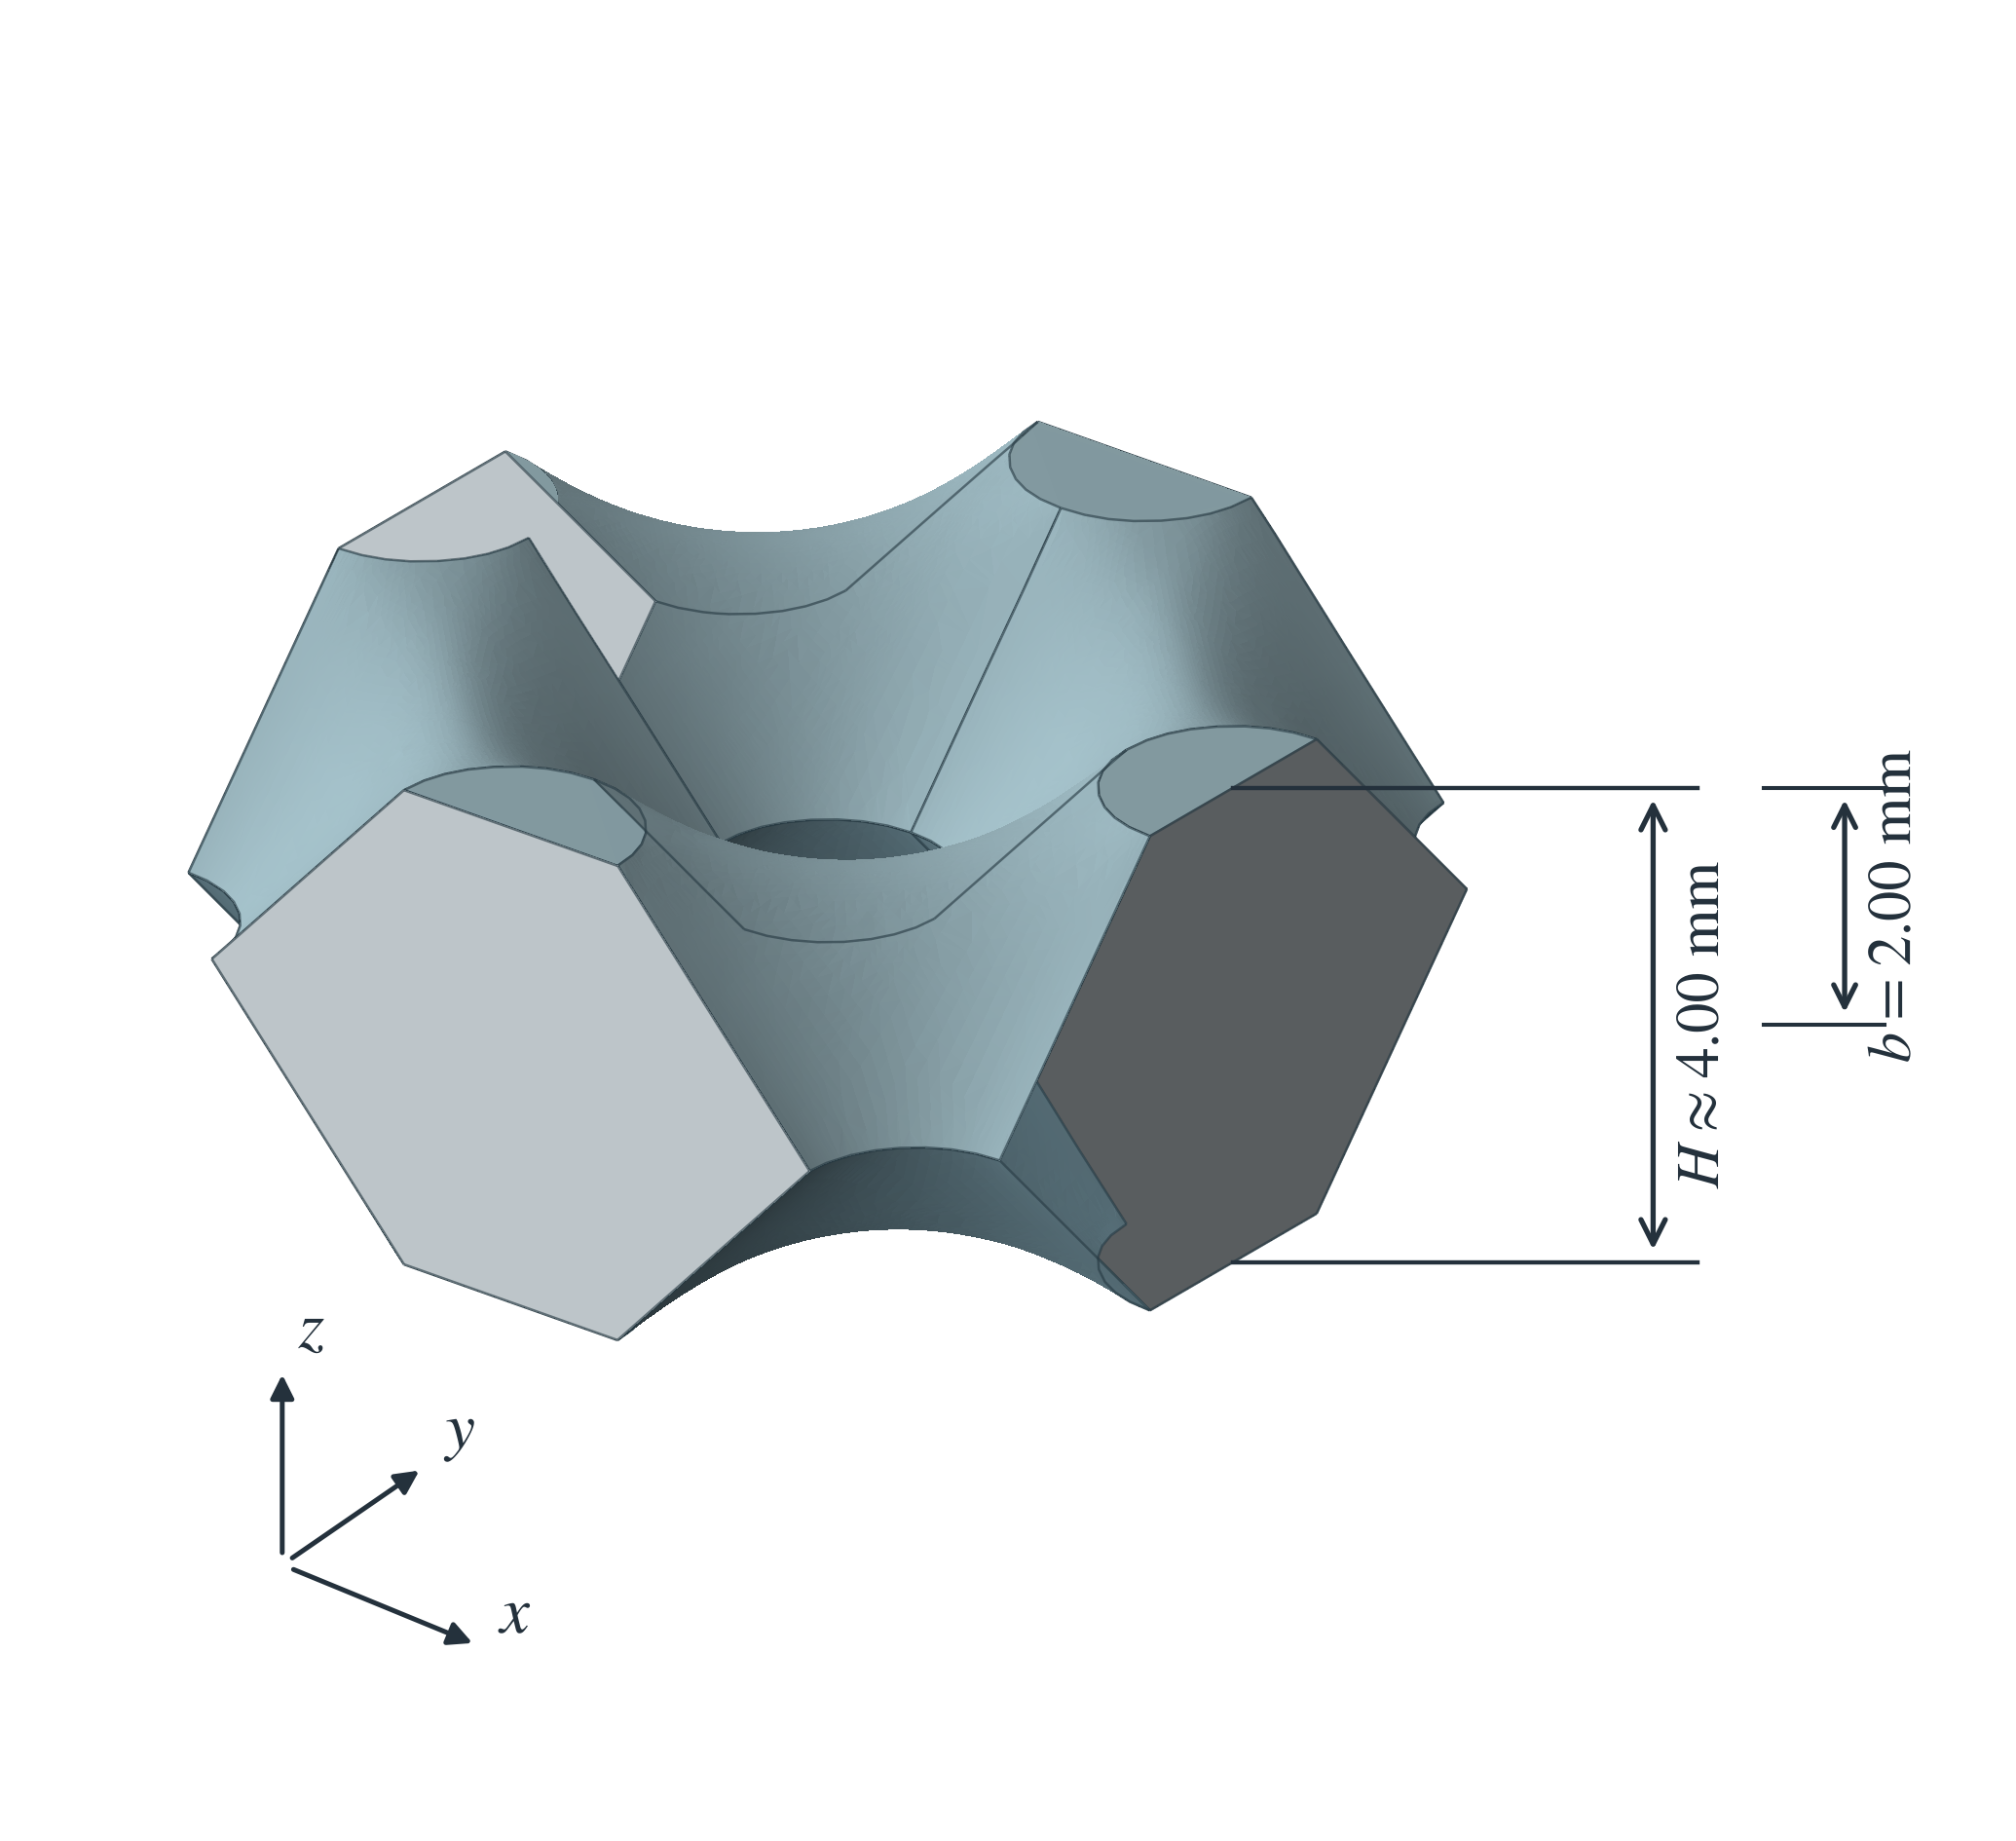
\includegraphics[width=\linewidth]{du_d3_geometry_iso.png}\par
    \small\textbf{(a)} Isometric fluid-domain view
  \end{minipage}\hfill
  \begin{minipage}[t]{0.49\linewidth}
    \centering
    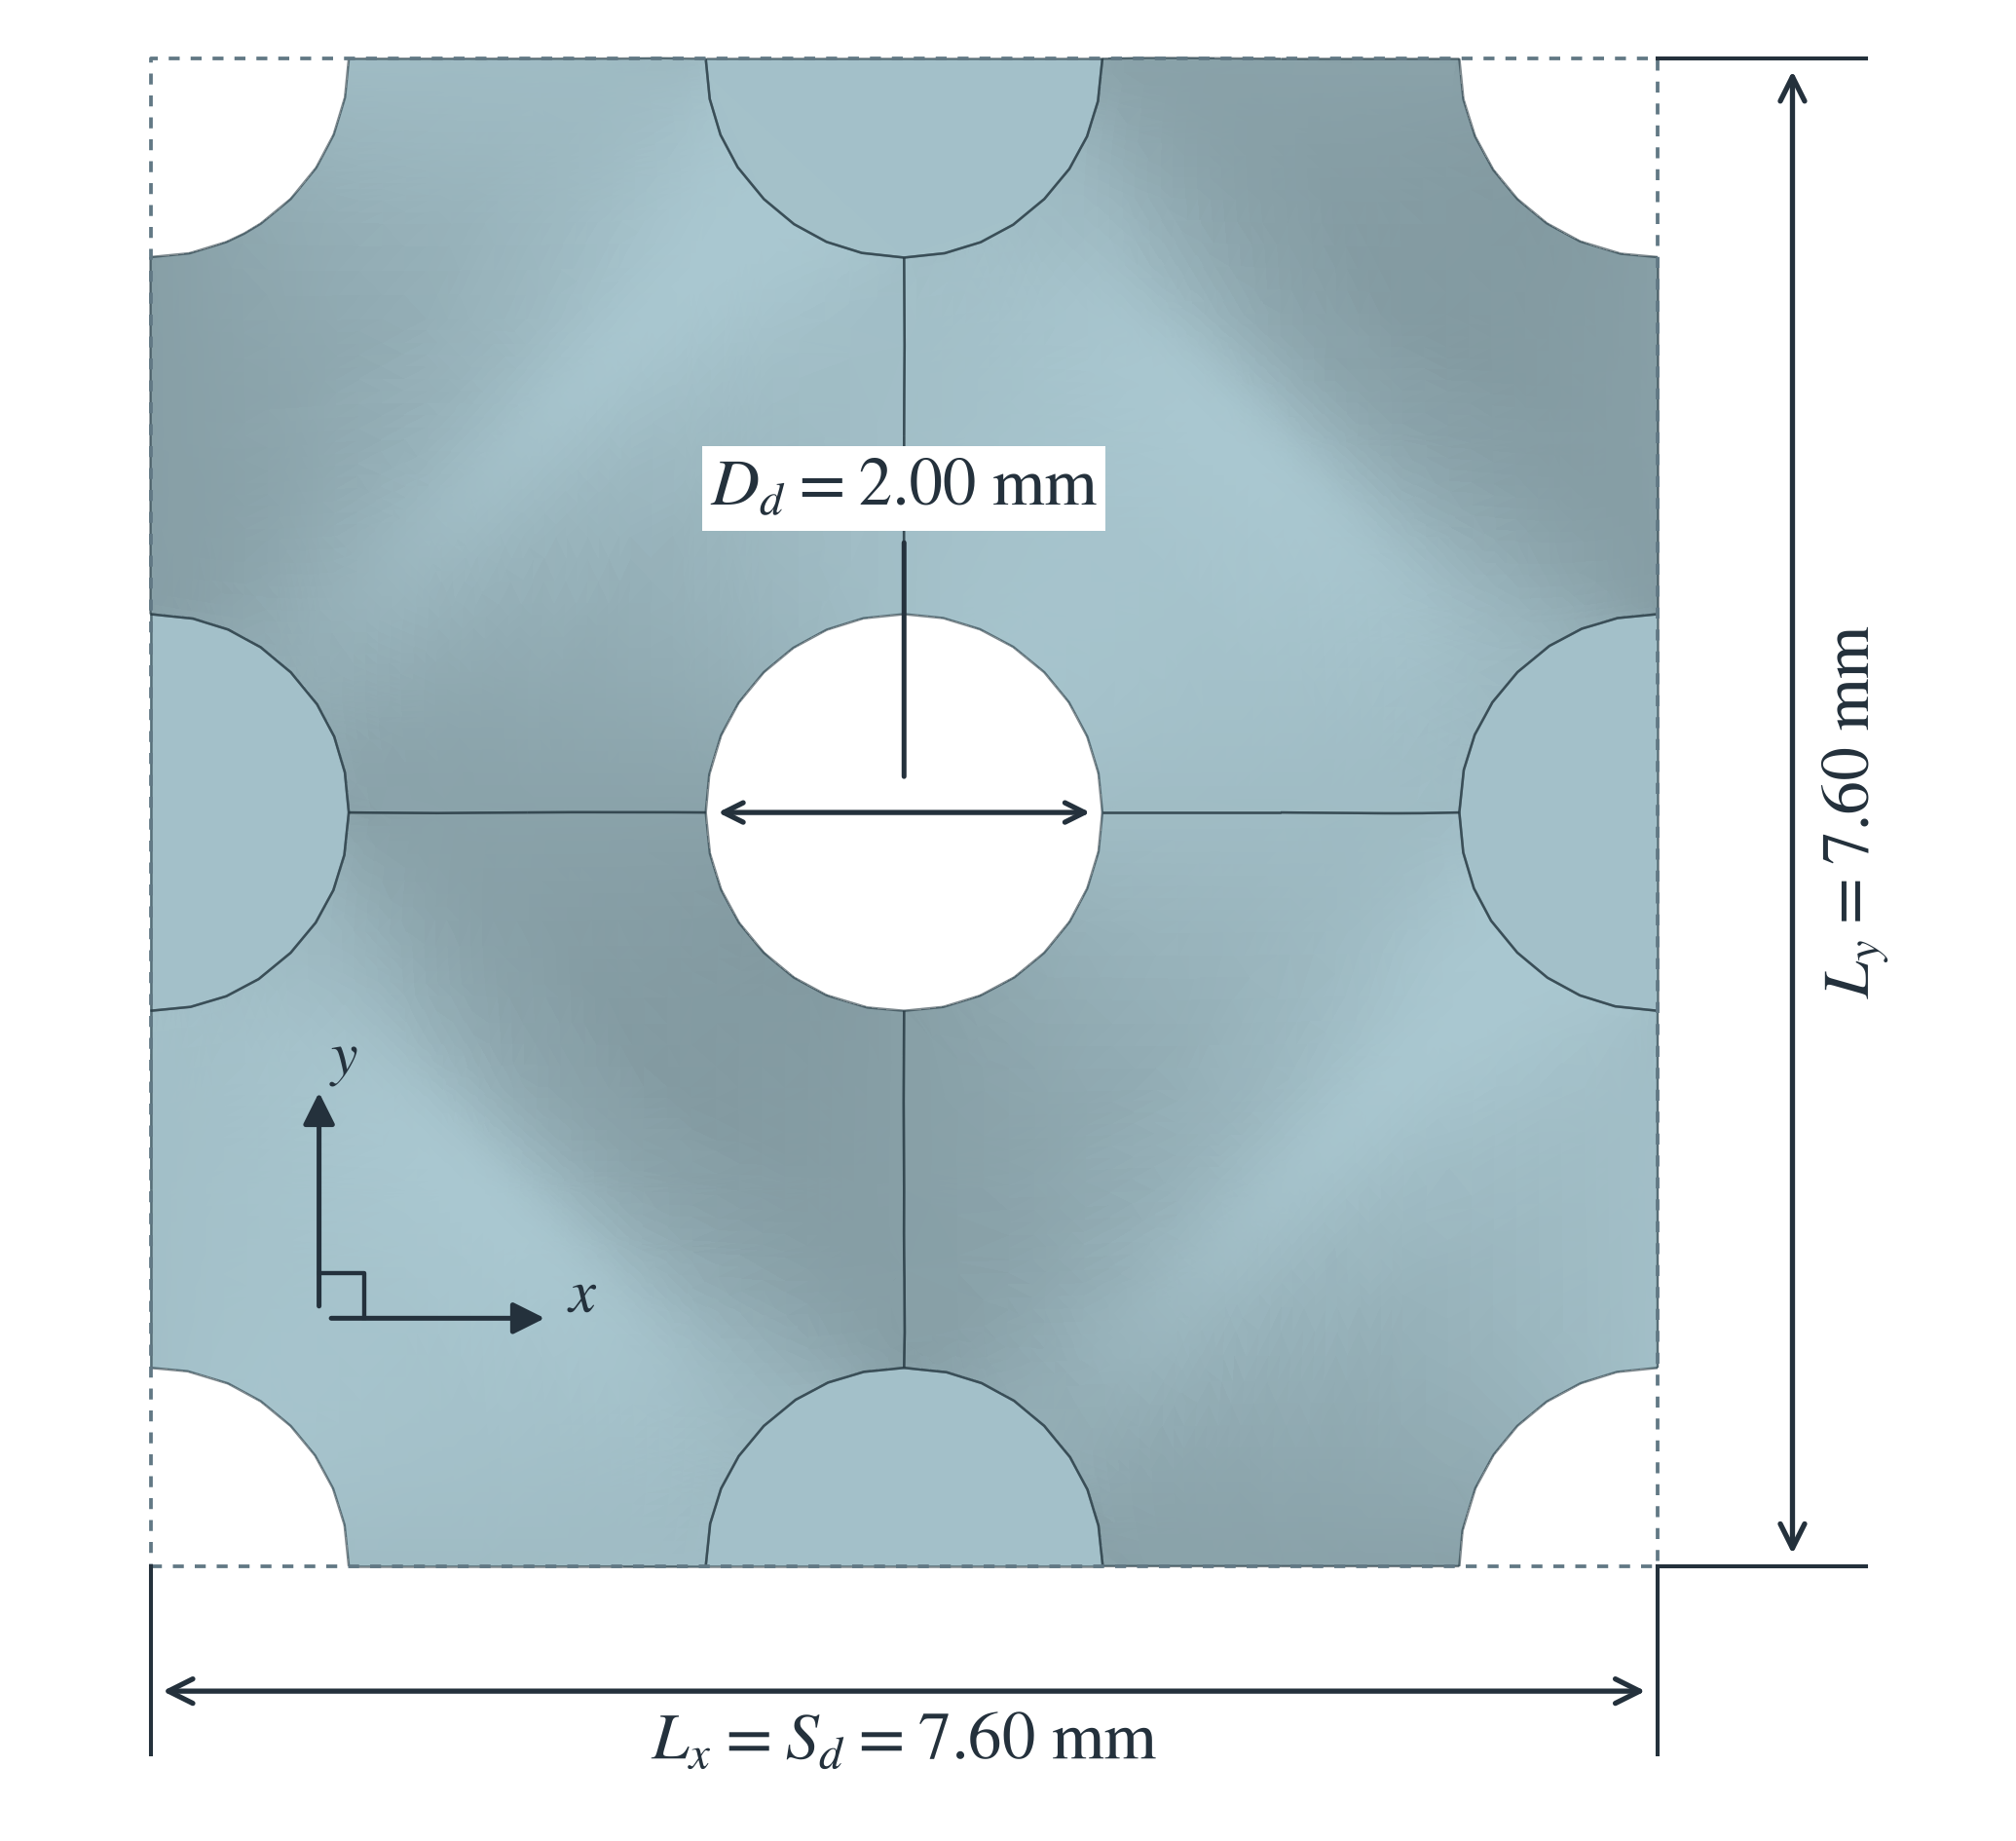
\includegraphics[width=\linewidth]{du_d3_geometry_plan.png}\par
    \small\textbf{(b)} Plan view and repeat dimensions
  \end{minipage}
  \caption{D3 validation unit cell visualised from the supplied CAD fluid domain: (a) isometric view with the nominal pressing depth $b$ and approximate full vertical envelope $H$; (b) plan view with repeat lengths $L_x$, $L_y$ and nominal dimple size $D_d$. Linear dimensions are in millimetres. $S_d$ is the reported dimple pitch. Colours distinguish geometric surfaces and are not solution fields; the central circular footprint is excluded from the fluid.}
  \label{fig:du-d3-geometry}
\end{figure}

\begin{table}[H]
  \centering
  \caption{Dimensions of the D3 benchmark geometry. Reported experimental dimensions follow \citet{du2025}, Table~3; CAD dimensions describe the supplied fluid-domain model. Nominal values are not manufacturing-tolerance or exact surface-matching claims.}
  \label{tab:du-d3-dimensions}
  \small
  \setlength{\tabcolsep}{4pt}
  \renewcommand{\arraystretch}{1.13}
  \begin{tabular}{@{}p{0.32\linewidth}cp{0.12\linewidth}p{0.39\linewidth}@{}}
    \hline
    \textbf{Quantity} & \textbf{Symbol} & \textbf{Value} & \textbf{Definition / source}\\
    \hline
    Unit-cell repeat lengths & $L_x,L_y$ & 7.60~mm & Opposing CAD cut-plane separations in $x$ and $y$.\\
    Dimple pitch & $S_d$ & 7.60~mm & Reported D3 pitch; matches the nominal cell repeat.\\
    Pressing depth & $b$ & 2.00~mm & Reported D3 pressing depth; nominal height from the contact plane to one wall extremum.\\
    Dimple size & $D_d$ & 2.00~mm & Reported D3 dimple size; central contact-footprint diameter in the plan view.\\
    Full vertical fluid envelope & $H$ & $\approx4.00$~mm & Approximate CAD span from $z\approx-2$ to $+2$~mm; not a uniform local channel gap.\\
    Dimple arrangement angle & $\beta$ & $90\degree$ & Reported D3 layout; distinct from the flow-entry angle.\\
    Solid plate thickness & $\delta_p$ & 0.25~mm & Reported experimental plate thickness.\\
    \hline
  \end{tabular}
\end{table}
